\section{Feature Detection}

\ifCPy

\cvCPyFunc{Canny}
Implements the Canny algorithm for edge detection.

\cvdefC{
void cvCanny(\par const CvArr* image,
\par CvArr* edges,
\par double threshold1,
\par double threshold2,
\par int aperture\_size=3 );
}\cvdefPy{Canny(image,edges,threshold1,threshold2,aperture\_size=3)-> None}
\begin{description}
\cvarg{image}{Single-channel input image}
\cvarg{edges}{Single-channel image to store the edges found by the function}
\cvarg{threshold1}{The first threshold}
\cvarg{threshold2}{The second threshold}
\cvarg{aperture\_size}{Aperture parameter for the Sobel operator (see \cvCPyCross{Sobel})}
\end{description}

The function finds the edges on the input image \texttt{image} and marks them in the output image \texttt{edges} using the Canny algorithm. The smallest value between \texttt{threshold1} and \texttt{threshold2} is used for edge linking, the largest value is used to find the initial segments of strong edges.

\cvCPyFunc{CornerEigenValsAndVecs}
Calculates eigenvalues and eigenvectors of image blocks for corner detection.

\cvdefC{
void cvCornerEigenValsAndVecs( \par const CvArr* image,\par CvArr* eigenvv,\par int blockSize,\par int aperture\_size=3 );

}\cvdefPy{CornerEigenValsAndVecs(image,eigenvv,blockSize,aperture\_size=3)-> None}

\begin{description}
\cvarg{image}{Input image}
\cvarg{eigenvv}{Image to store the results. It must be 6 times wider than the input image}
\cvarg{blockSize}{Neighborhood size (see discussion)}
\cvarg{aperture\_size}{Aperture parameter for the Sobel operator (see \cvCPyCross{Sobel})}
\end{description}

For every pixel, the function \texttt{cvCornerEigenValsAndVecs} considers a $\texttt{blockSize} \times \texttt{blockSize}$ neigborhood S(p). It calcualtes the covariation matrix of derivatives over the neigborhood as:

\[
M = \begin{bmatrix}
\sum_{S(p)}(dI/dx)^2 & \sum_{S(p)}(dI/dx \cdot dI/dy)^2 \\
\sum_{S(p)}(dI/dx \cdot dI/dy)^2 & \sum_{S(p)}(dI/dy)^2
\end{bmatrix}
\]

After that it finds eigenvectors and eigenvalues of the matrix and stores them into destination image in form
$(\lambda_1, \lambda_2, x_1, y_1, x_2, y_2)$ where
\begin{description}
\item[$\lambda_1, \lambda_2$]are the eigenvalues of $M$; not sorted
\item[$x_1, y_1$]are the eigenvectors corresponding to $\lambda_1$
\item[$x_2, y_2$]are the eigenvectors corresponding to $\lambda_2$
\end{description}

\cvCPyFunc{CornerHarris}
Harris edge detector.

\cvdefC{
void cvCornerHarris(
\par const CvArr* image,
\par CvArr* harris\_responce,
\par int blockSize,
\par int aperture\_size=3,
\par double k=0.04 );
}\cvdefPy{CornerHarris(image,harris\_dst,blockSize,aperture\_size=3,k=0.04)-> None}

\begin{description}
\cvarg{image}{Input image}
\cvarg{harris\_responce}{Image to store the Harris detector responses. Should have the same size as \texttt{image}}
\cvarg{blockSize}{Neighborhood size (see the discussion of \cvCPyCross{CornerEigenValsAndVecs})}
\cvarg{aperture\_size}{Aperture parameter for the Sobel operator (see \cvCPyCross{Sobel}).}
% format. In the case of floating-point input format this parameter is the number of the fixed float filter used for differencing
\cvarg{k}{Harris detector free parameter. See the formula below}
\end{description}

The function runs the Harris edge detector on the image. Similarly to \cvCPyCross{CornerMinEigenVal} and \cvCPyCross{CornerEigenValsAndVecs}, for each pixel it calculates a $2\times2$ gradient covariation matrix $M$ over a $\texttt{blockSize} \times \texttt{blockSize}$ neighborhood. Then, it stores

\[
det(M) - k \, trace(M)^2
\]

to the destination image. Corners in the image can be found as the local maxima of the destination image.

\cvCPyFunc{CornerMinEigenVal}
Calculates the minimal eigenvalue of gradient matrices for corner detection.

\cvdefC{
void cvCornerMinEigenVal(
\par const CvArr* image,
\par CvArr* eigenval,
\par int blockSize,
\par int aperture\_size=3 );
}\cvdefPy{CornerMinEigenVal(image,eigenval,blockSize,aperture\_size=3)-> None}
\begin{description}
\cvarg{image}{Input image}
\cvarg{eigenval}{Image to store the minimal eigenvalues. Should have the same size as \texttt{image}}
\cvarg{blockSize}{Neighborhood size (see the discussion of \cvCPyCross{CornerEigenValsAndVecs})}
\cvarg{aperture\_size}{Aperture parameter for the Sobel operator (see \cvCPyCross{Sobel}).}
%  format. In the case of floating-point input format this parameter is the number of the fixed float filter used for differencing
\end{description}

The function is similar to \cvCPyCross{CornerEigenValsAndVecs} but it calculates and stores only the minimal eigen value of derivative covariation matrix for every pixel, i.e. $min(\lambda_1, \lambda_2)$ in terms of the previous function.

\cvCPyFunc{ExtractSURF}
Extracts Speeded Up Robust Features from an image.

\cvdefC{
void cvExtractSURF( \par const CvArr* image,\par const CvArr* mask,\par CvSeq** keypoints,\par CvSeq** descriptors,\par CvMemStorage* storage,\par CvSURFParams params );
}\cvdefPy{ExtractSURF(image,mask,storage,params)-> keypoints,descriptors}

\begin{description}
\cvarg{image}{The input 8-bit grayscale image}
\cvarg{mask}{The optional input 8-bit mask. The features are only found in the areas that contain more than 50\% of non-zero mask pixels}
\cvarg{keypoints}{The output parameter; double pointer to the sequence of keypoints. The sequence of CvSURFPoint structures is as follows:}
\begin{lstlisting}
 typedef struct CvSURFPoint
 {
    CvPoint2D32f pt; // position of the feature within the image
    int laplacian;   // -1, 0 or +1. sign of the laplacian at the point.
                     // can be used to speedup feature comparison
                     // (normally features with laplacians of different 
             // signs can not match)
    int size;        // size of the feature
    float dir;       // orientation of the feature: 0..360 degrees
    float hessian;   // value of the hessian (can be used to 
             // approximately estimate the feature strengths;
                     // see also params.hessianThreshold)
 }
 CvSURFPoint;
\end{lstlisting}
\cvarg{descriptors}{The optional output parameter; double pointer to the sequence of descriptors. Depending on the params.extended value, each element of the sequence will be either a 64-element or a 128-element floating-point (\texttt{CV\_32F}) vector. If the parameter is NULL, the descriptors are not computed}
\cvarg{storage}{Memory storage where keypoints and descriptors will be stored}
\cvarg{params}{Various algorithm parameters put to the structure CvSURFParams:}
\begin{lstlisting}
 typedef struct CvSURFParams
 {
    int extended; // 0 means basic descriptors (64 elements each),
                  // 1 means extended descriptors (128 elements each)
    double hessianThreshold; // only features with keypoint.hessian 
          // larger than that are extracted.
                  // good default value is ~300-500 (can depend on the 
          // average local contrast and sharpness of the image).
                  // user can further filter out some features based on 
          // their hessian values and other characteristics.
    int nOctaves; // the number of octaves to be used for extraction.
                  // With each next octave the feature size is doubled 
          // (3 by default)
    int nOctaveLayers; // The number of layers within each octave 
          // (4 by default)
 }
 CvSURFParams;

 CvSURFParams cvSURFParams(double hessianThreshold, int extended=0); 
          // returns default parameters
\end{lstlisting}
\end{description}

The function cvExtractSURF finds robust features in the image, as
described in
Bay06
. For each feature it returns its location, size,
orientation and optionally the descriptor, basic or extended. The function
can be used for object tracking and localization, image stitching etc. See the
\texttt{find\_obj.cpp} demo in OpenCV samples directory.

\cvCPyFunc{FindCornerSubPix}
Refines the corner locations.

\cvdefC{
void cvFindCornerSubPix(
\par const CvArr* image,
\par CvPoint2D32f* corners,
\par int count,
\par CvSize win,
\par CvSize zero\_zone,
\par CvTermCriteria criteria );
}\cvdefPy{FindCornerSubPix(image,corners,win,zero\_zone,criteria)-> corners}

\begin{description}
\cvarg{image}{Input image}
\ifC
\cvarg{corners}{Initial coordinates of the input corners; refined coordinates on output}
\cvarg{count}{Number of corners}
\fi
\ifPy
\cvarg{corners}{Initial coordinates of the input corners as a list of (x, y) pairs}
\fi
\cvarg{win}{Half of the side length of the search window. For example, if \texttt{win}=(5,5), then a $5*2+1 \times 5*2+1 = 11 \times 11$ search window would be used}
\cvarg{zero\_zone}{Half of the size of the dead region in the middle of the search zone over which the summation in the formula below is not done. It is used sometimes to avoid possible singularities of the autocorrelation matrix. The value of (-1,-1) indicates that there is no such size}
\cvarg{criteria}{Criteria for termination of the iterative process of corner refinement. That is, the process of corner position refinement stops either after a certain number of iterations or when a required accuracy is achieved. The \texttt{criteria} may specify either of or both the maximum number of iteration and the required accuracy}
\end{description}

The function iterates to find the sub-pixel accurate location of corners, or radial saddle points, as shown in on the picture below.
\ifPy
It returns the refined coordinates as a list of (x, y) pairs.
\fi

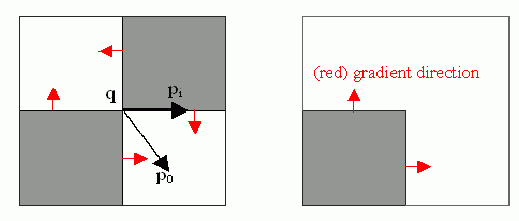
\includegraphics[width=1.0\textwidth]{pics/cornersubpix.png}

Sub-pixel accurate corner locator is based on the observation that every vector from the center $q$ to a point $p$ located within a neighborhood of $q$ is orthogonal to the image gradient at $p$ subject to image and measurement noise. Consider the expression:

\[
\epsilon_i = {DI_{p_i}}^T \cdot (q - p_i)
\]

where ${DI_{p_i}}$ is the image gradient at the one of the points $p_i$ in a neighborhood of $q$. The value of $q$ is to be found such that $\epsilon_i$ is minimized. A system of equations may be set up with $\epsilon_i$ set to zero:

\[
\sum_i(DI_{p_i} \cdot {DI_{p_i}}^T) q = \sum_i(DI_{p_i} \cdot {DI_{p_i}}^T \cdot p_i)
\]

where the gradients are summed within a neighborhood ("search window") of $q$. Calling the first gradient term $G$ and the second gradient term $b$ gives:

\[
q = G^{-1} \cdot b
\]

The algorithm sets the center of the neighborhood window at this new center $q$ and then iterates until the center keeps within a set threshold.

\cvCPyFunc{GetStarKeypoints}
Retrieves keypoints using the StarDetector algorithm.

\cvdefC{
CvSeq* cvGetStarKeypoints( \par const CvArr* image,\par CvMemStorage* storage,\par CvStarDetectorParams params=cvStarDetectorParams() );
}\cvdefPy{GetStarKeypoints(image,storage,params)-> keypoints}

\begin{description}
\cvarg{image}{The input 8-bit grayscale image}
\cvarg{storage}{Memory storage where the keypoints will be stored}
\cvarg{params}{Various algorithm parameters given to the structure CvStarDetectorParams:}
\begin{lstlisting}
 typedef struct CvStarDetectorParams
 {
    int maxSize; // maximal size of the features detected. The following 
                 // values of the parameter are supported:
                 // 4, 6, 8, 11, 12, 16, 22, 23, 32, 45, 46, 64, 90, 128
    int responseThreshold; // threshold for the approximatd laplacian,
                           // used to eliminate weak features
    int lineThresholdProjected; // another threshold for laplacian to 
                // eliminate edges
    int lineThresholdBinarized; // another threshold for the feature 
                // scale to eliminate edges
    int suppressNonmaxSize; // linear size of a pixel neighborhood 
                // for non-maxima suppression
 }
 CvStarDetectorParams;
\end{lstlisting}
\end{description}

The function GetStarKeypoints extracts keypoints that are local
scale-space extremas. The scale-space is constructed by computing
approximate values of laplacians with different sigma's at each
pixel. Instead of using pyramids, a popular approach to save computing
time, all of the laplacians are computed at each pixel of the original
high-resolution image. But each approximate laplacian value is computed
in O(1) time regardless of the sigma, thanks to the use of integral
images. The algorithm is based on the paper 
Agrawal08
, but instead
of a square, hexagon or octagon it uses an 8-end star shape, hence the name,
consisting of overlapping upright and tilted squares.

Each computed feature is represented by the following structure:

\begin{lstlisting}
typedef struct CvStarKeypoint
{
    CvPoint pt; // coordinates of the feature
    int size; // feature size, see CvStarDetectorParams::maxSize
    float response; // the approximated laplacian value at that point.
}
CvStarKeypoint;

inline CvStarKeypoint cvStarKeypoint(CvPoint pt, int size, float response);
\end{lstlisting}

\ifC
Below is the small usage sample:

\begin{lstlisting}
#include "cv.h"
#include "highgui.h"

int main(int argc, char** argv)
{
    const char* filename = argc > 1 ? argv[1] : "lena.jpg";
    IplImage* img = cvLoadImage( filename, 0 ), *cimg;
    CvMemStorage* storage = cvCreateMemStorage(0);
    CvSeq* keypoints = 0;
    int i;

    if( !img )
        return 0;
    cvNamedWindow( "image", 1 );
    cvShowImage( "image", img );
    cvNamedWindow( "features", 1 );
    cimg = cvCreateImage( cvGetSize(img), 8, 3 );
    cvCvtColor( img, cimg, CV_GRAY2BGR );

    keypoints = cvGetStarKeypoints( img, storage, cvStarDetectorParams(45) );

    for( i = 0; i < (keypoints ? keypoints->total : 0); i++ )
    {
        CvStarKeypoint kpt = *(CvStarKeypoint*)cvGetSeqElem(keypoints, i);
        int r = kpt.size/2;
        cvCircle( cimg, kpt.pt, r, CV_RGB(0,255,0));
        cvLine( cimg, cvPoint(kpt.pt.x + r, kpt.pt.y + r),
            cvPoint(kpt.pt.x - r, kpt.pt.y - r), CV_RGB(0,255,0));
        cvLine( cimg, cvPoint(kpt.pt.x - r, kpt.pt.y + r),
            cvPoint(kpt.pt.x + r, kpt.pt.y - r), CV_RGB(0,255,0));
    }
    cvShowImage( "features", cimg );
    cvWaitKey();
}
\end{lstlisting}
\fi

\cvCPyFunc{GoodFeaturesToTrack}
Determines strong corners on an image.

\cvdefC{
void cvGoodFeaturesToTrack(
\par const CvArr* image
\par CvArr* eigImage, CvArr* tempImage
\par CvPoint2D32f* corners
\par int* cornerCount
\par double qualityLevel
\par double minDistance
\par const CvArr* mask=NULL
\par int blockSize=3
\par int useHarris=0
\par double k=0.04 );
}
\cvdefPy{GoodFeaturesToTrack(image,eigImage,tempImage,qualityLevel,minDistance,mask=NULL,blockSize=3,useHarris=0,k=0.04)-> corners}

\begin{description}
\cvarg{image}{The source 8-bit or floating-point 32-bit, single-channel image}
\cvarg{eigImage}{Temporary floating-point 32-bit image, the same size as \texttt{image}}
\cvarg{tempImage}{Another temporary image, the same size and format as \texttt{eigImage}}
\cvarg{corners}{Output parameter; detected corners}
\cvarg{cornerCount}{Output parameter; number of detected corners}
\cvarg{qualityLevel}{Multiplier for the max/min eigenvalue; specifies the minimal accepted quality of image corners}
\cvarg{minDistance}{Limit, specifying the minimum possible distance between the returned corners; Euclidian distance is used}
\cvarg{mask}{Region of interest. The function selects points either in the specified region or in the whole image if the mask is NULL}
\cvarg{blockSize}{Size of the averaging block, passed to the underlying \cvCPyCross{CornerMinEigenVal} or \cvCPyCross{CornerHarris} used by the function}
\cvarg{useHarris}{If nonzero, Harris operator (\cvCPyCross{CornerHarris}) is used instead of default \cvCPyCross{CornerMinEigenVal}}
\cvarg{k}{Free parameter of Harris detector; used only if ($\texttt{useHarris} != 0$)}
\end{description}

The function finds the corners with big eigenvalues in the image. The function first calculates the minimal
eigenvalue for every source image pixel using the \cvCPyCross{CornerMinEigenVal}
function and stores them in \texttt{eigImage}. Then it performs
non-maxima suppression (only the local maxima in $3\times 3$ neighborhood
are retained). The next step rejects the corners with the minimal
eigenvalue less than $\texttt{qualityLevel} \cdot max(\texttt{eigImage}(x,y))$.
Finally, the function ensures that the distance between any two corners is not smaller than \texttt{minDistance}. The weaker corners (with a smaller min eigenvalue) that are too close to the stronger corners are rejected.

Note that the if the function is called with different values \texttt{A} and \texttt{B} of the parameter \texttt{qualityLevel}, and \texttt{A} > {B}, the array of returned corners with \texttt{qualityLevel=A} will be the prefix of the output corners array with \texttt{qualityLevel=B}.

\cvCPyFunc{HoughLines2}
Finds lines in a binary image using a Hough transform.

\cvdefC{
CvSeq* cvHoughLines2( \par CvArr* image,\par void* line\_storage,\par int method,\par double rho,\par double theta,\par int threshold,\par double param1=0,\par double param2=0 );
}\cvdefPy{HoughLines2(image,storage,method,rho,theta,threshold,param1=0,parma2=0)-> lines}

\begin{description}
\cvarg{image}{The 8-bit, single-channel, binary source image. In the case of a probabilistic method, the image is modified by the function}
\cvarg{line\_storage}{The storage for the lines that are detected. It can
be a memory storage (in this case a sequence of lines is created in
the storage and returned by the function) or single row/single column
matrix (CvMat*) of a particular type (see below) to which the lines'
parameters are written. The matrix header is modified by the function
so its \texttt{cols} or \texttt{rows} will contain the number of lines
detected. If \texttt{line\_storage} is a matrix and the actual number
of lines exceeds the matrix size, the maximum possible number of lines
is returned (in the case of standard hough transform the lines are sorted
by the accumulator value)}
\cvarg{method}{The Hough transform variant, one of the following:
\begin{description}
  \cvarg{CV\_HOUGH\_STANDARD}{classical or standard Hough transform. Every line is represented by two floating-point numbers $(\rho, \theta)$, where $\rho$ is a distance between (0,0) point and the line, and $\theta$ is the angle between x-axis and the normal to the line. Thus, the matrix must be (the created sequence will be) of \texttt{CV\_32FC2} type}
  \cvarg{CV\_HOUGH\_PROBABILISTIC}{probabilistic Hough transform (more efficient in case if picture contains a few long linear segments). It returns line segments rather than the whole line. Each segment is represented by starting and ending points, and the matrix must be (the created sequence will be) of \texttt{CV\_32SC4} type}
  \cvarg{CV\_HOUGH\_MULTI\_SCALE}{multi-scale variant of the classical Hough transform. The lines are encoded the same way as \texttt{CV\_HOUGH\_STANDARD}}
\end{description}}
\cvarg{rho}{Distance resolution in pixel-related units}
\cvarg{theta}{Angle resolution measured in radians}
\cvarg{threshold}{Threshold parameter. A line is returned by the function if the corresponding accumulator value is greater than \texttt{threshold}}
\cvarg{param1}{The first method-dependent parameter:
\begin{itemize}
  \item For the classical Hough transform it is not used (0).
  \item For the probabilistic Hough transform it is the minimum line length.
  \item For the multi-scale Hough transform it is the divisor for the distance resolution $\rho$. (The coarse distance resolution will be $\rho$ and the accurate resolution will be $(\rho / \texttt{param1})$).
\end{itemize}}
\cvarg{param2}{The second method-dependent parameter:
\begin{itemize}
  \item For the classical Hough transform it is not used (0).
  \item For the probabilistic Hough transform it is the maximum gap between line segments lying on the same line to treat them as a single line segment (i.e. to join them).
  \item For the multi-scale Hough transform it is the divisor for the angle resolution $\theta$. (The coarse angle resolution will be $\theta$ and the accurate resolution will be $(\theta / \texttt{param2})$).
\end{itemize}}
\end{description}

The function implements a few variants of the Hough transform for line detection.

\ifC
\textbf{Example. Detecting lines with Hough transform.}
\begin{lstlisting}
/* This is a standalone program. Pass an image name as a first parameter
of the program.  Switch between standard and probabilistic Hough transform
by changing "#if 1" to "#if 0" and back */
#include <cv.h>
#include <highgui.h>
#include <math.h>

int main(int argc, char** argv)
{
    IplImage* src;
    if( argc == 2 && (src=cvLoadImage(argv[1], 0))!= 0)
    {
        IplImage* dst = cvCreateImage( cvGetSize(src), 8, 1 );
        IplImage* color_dst = cvCreateImage( cvGetSize(src), 8, 3 );
        CvMemStorage* storage = cvCreateMemStorage(0);
        CvSeq* lines = 0;
        int i;
        cvCanny( src, dst, 50, 200, 3 );
        cvCvtColor( dst, color_dst, CV_GRAY2BGR );
#if 1
        lines = cvHoughLines2( dst,
                               storage,
                               CV_HOUGH_STANDARD,
                               1,
                               CV_PI/180,
                               100,
                               0,
                               0 );

        for( i = 0; i < MIN(lines->total,100); i++ )
        {
            float* line = (float*)cvGetSeqElem(lines,i);
            float rho = line[0];
            float theta = line[1];
            CvPoint pt1, pt2;
            double a = cos(theta), b = sin(theta);
            double x0 = a*rho, y0 = b*rho;
            pt1.x = cvRound(x0 + 1000*(-b));
            pt1.y = cvRound(y0 + 1000*(a));
            pt2.x = cvRound(x0 - 1000*(-b));
            pt2.y = cvRound(y0 - 1000*(a));
            cvLine( color_dst, pt1, pt2, CV_RGB(255,0,0), 3, 8 );
        }
#else
        lines = cvHoughLines2( dst,
                               storage,
                               CV_HOUGH_PROBABILISTIC,
                               1,
                               CV_PI/180,
                               80,
                               30,
                               10 );
        for( i = 0; i < lines->total; i++ )
        {
            CvPoint* line = (CvPoint*)cvGetSeqElem(lines,i);
            cvLine( color_dst, line[0], line[1], CV_RGB(255,0,0), 3, 8 );
        }
#endif
        cvNamedWindow( "Source", 1 );
        cvShowImage( "Source", src );

        cvNamedWindow( "Hough", 1 );
        cvShowImage( "Hough", color_dst );

        cvWaitKey(0);
    }
}
\end{lstlisting}

This is the sample picture the function parameters have been tuned for:

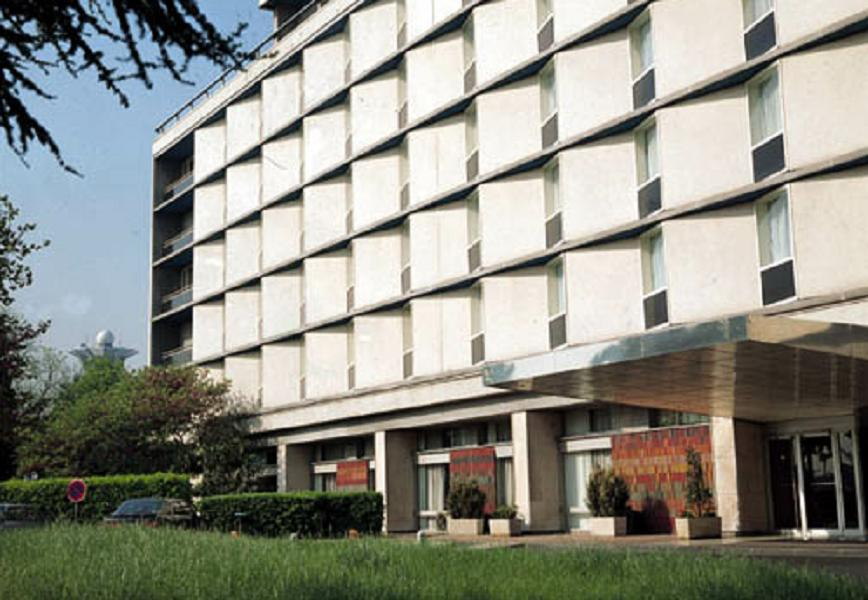
\includegraphics[width=0.5\textwidth]{pics/building.jpg}

And this is the output of the above program in the case of probabilistic Hough transform (\texttt{\#if 0} case):

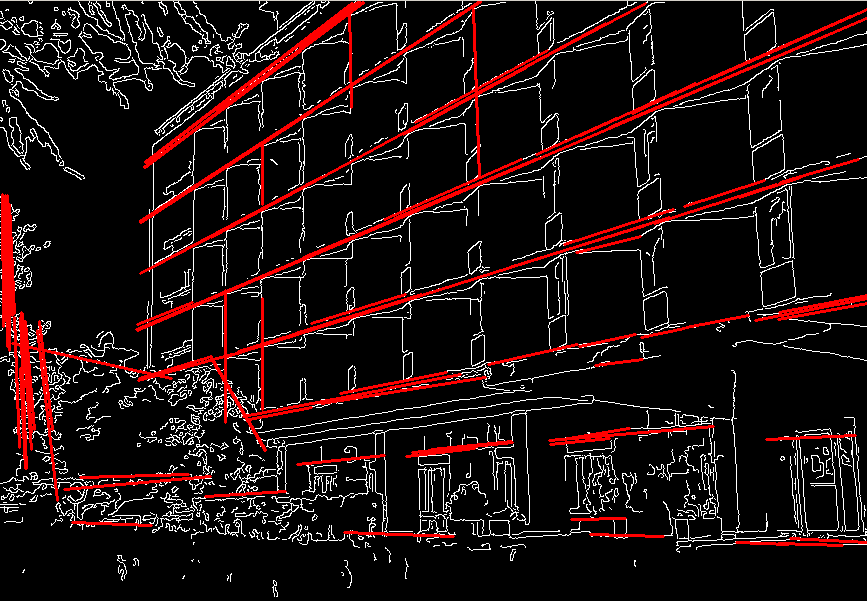
\includegraphics[width=0.5\textwidth]{pics/houghp.png}
\fi

\cvCPyFunc{PreCornerDetect}
Calculates the feature map for corner detection.

\cvdefC{
void cvPreCornerDetect(
\par const CvArr* image,
\par CvArr* corners,
\par int apertureSize=3 );
}\cvdefPy{PreCornerDetect(image,corners,aperture\_size=3)-> None}
\begin{description}
\cvarg{image}{Input image}
\cvarg{corners}{Image to store the corner candidates}
\cvarg{apertureSize}{Aperture parameter for the Sobel operator (see \cvCPyCross{Sobel})}
\end{description}

The function calculates the function

\[
D_x^2 D_{yy} + D_y^2 D_{xx} - 2 D_x D_y D_{xy}
\]

where $D_?$ denotes one of the first image derivatives and $D_{??}$ denotes a second image derivative.

The corners can be found as local maximums of the function below:

\begin{lstlisting}
// assume that the image is floating-point
IplImage* corners = cvCloneImage(image);
IplImage* dilated_corners = cvCloneImage(image);
IplImage* corner_mask = cvCreateImage( cvGetSize(image), 8, 1 );
cvPreCornerDetect( image, corners, 3 );
cvDilate( corners, dilated_corners, 0, 1 );
cvSubS( corners, dilated_corners, corners );
cvCmpS( corners, 0, corner_mask, CV_CMP_GE );
cvReleaseImage( &corners );
cvReleaseImage( &dilated_corners );
\end{lstlisting}

\ifC
\cvCPyFunc{SampleLine}
Reads the raster line to the buffer.

\cvdefC{
int cvSampleLine(
\par const CvArr* image
\par CvPoint pt1
\par CvPoint pt2
\par void* buffer
\par int connectivity=8 );
}

\begin{description}
\cvarg{image}{Image to sample the line from}
\cvarg{pt1}{Starting line point}
\cvarg{pt2}{Ending line point}
\cvarg{buffer}{Buffer to store the line points; must have enough size to store
$max( |\texttt{pt2.x} - \texttt{pt1.x}|+1, |\texttt{pt2.y} - \texttt{pt1.y}|+1 )$
points in the case of an 8-connected line and
$ (|\texttt{pt2.x}-\texttt{pt1.x}|+|\texttt{pt2.y}-\texttt{pt1.y}|+1) $
in the case of a 4-connected line}
\cvarg{connectivity}{The line connectivity, 4 or 8}
\end{description}

The function implements a particular application of line iterators. The function reads all of the image points lying on the line between \texttt{pt1} and \texttt{pt2}, including the end points, and stores them into the buffer.

\fi

\fi


\ifCpp

\cvCppFunc{Canny}
Finds edges in an image using Canny algorithm.

\cvdefCpp{void Canny( const Mat\& image, Mat\& edges,\par
            double threshold1, double threshold2,\par
            int apertureSize=3, bool L2gradient=false );}
\begin{description}
\cvarg{image}{Single-channel 8-bit input image}
\cvarg{edges}{The output edge map. It will have the same size and the same type as \texttt{image}}
\cvarg{threshold1}{The first threshold for the hysteresis procedure}
\cvarg{threshold2}{The second threshold for the hysteresis procedure}
\cvarg{apertureSize}{Aperture size for the \cvCppCross{Sobel} operator}
\cvarg{L2gradient}{Indicates, whether the more accurate $L_2$ norm $=\sqrt{(dI/dx)^2 + (dI/dy)^2}$ should be used to compute the image gradient magnitude (\texttt{L2gradient=true}), or a faster default $L_1$ norm $=|dI/dx|+|dI/dy|$ is enough (\texttt{L2gradient=false})}
\end{description}

The function finds edges in the input image \texttt{image} and marks them in the output map \texttt{edges} using the Canny algorithm. The smallest value between \texttt{threshold1} and \texttt{threshold2} is used for edge linking, the largest value is used to find the initial segments of strong edges, see
\url{http://en.wikipedia.org/wiki/Canny_edge_detector}

\cvCppFunc{cornerEigenValsAndVecs}
Calculates eigenvalues and eigenvectors of image blocks for corner detection.

\cvdefCpp{void cornerEigenValsAndVecs( const Mat\& src, Mat\& dst,\par
                            int blockSize, int apertureSize,\par
                            int borderType=BORDER\_DEFAULT );}
\begin{description}
\cvarg{src}{Input single-channel 8-bit or floating-point image}
\cvarg{dst}{Image to store the results. It will have the same size as \texttt{src} and the type \texttt{CV\_32FC(6)}}
\cvarg{blockSize}{Neighborhood size (see discussion)}
\cvarg{apertureSize}{Aperture parameter for the \cvCppCross{Sobel} operator}
\cvarg{boderType}{Pixel extrapolation method; see \cvCppCross{borderInterpolate}}
\end{description}

For every pixel $p$, the function \texttt{cornerEigenValsAndVecs} considers a \texttt{blockSize} $\times$ \texttt{blockSize} neigborhood $S(p)$. It calculates the covariation matrix of derivatives over the neighborhood as:

\[
M = \begin{bmatrix}
\sum_{S(p)}(dI/dx)^2 & \sum_{S(p)}(dI/dx dI/dy)^2 \\
\sum_{S(p)}(dI/dx dI/dy)^2 & \sum_{S(p)}(dI/dy)^2
\end{bmatrix}
\]

Where the derivatives are computed using \cvCppCross{Sobel} operator.

After that it finds eigenvectors and eigenvalues of $M$ and stores them into destination image in the form
$(\lambda_1, \lambda_2, x_1, y_1, x_2, y_2)$ where
\begin{description}
\item[$\lambda_1, \lambda_2$]are the eigenvalues of $M$; not sorted
\item[$x_1, y_1$]are the eigenvectors corresponding to $\lambda_1$
\item[$x_2, y_2$]are the eigenvectors corresponding to $\lambda_2$
\end{description}

The output of the function can be used for robust edge or corner detection.

See also: \cvCppCross{cornerMinEigenVal}, \cvCppCross{cornerHarris}, \cvCppCross{preCornerDetect}

\cvCppFunc{cornerHarris}
Harris edge detector.

\cvdefCpp{void cornerHarris( const Mat\& src, Mat\& dst, int blockSize,\par
                  int apertureSize, double k,\par
                  int borderType=BORDER\_DEFAULT );}
\begin{description}
\cvarg{src}{Input single-channel 8-bit or floating-point image}
\cvarg{dst}{Image to store the Harris detector responses; will have type \texttt{CV\_32FC1} and the same size as \texttt{src}}
\cvarg{blockSize}{Neighborhood size (see the discussion of \cvCppCross{cornerEigenValsAndVecs})}
\cvarg{apertureSize}{Aperture parameter for the \cvCppCross{Sobel} operator}
\cvarg{k}{Harris detector free parameter. See the formula below}
\cvarg{boderType}{Pixel extrapolation method; see \cvCppCross{borderInterpolate}}
\end{description}

The function runs the Harris edge detector on the image. Similarly to \cvCppCross{cornerMinEigenVal} and \cvCppCross{cornerEigenValsAndVecs}, for each pixel $(x, y)$ it calculates a $2\times2$ gradient covariation matrix $M^{(x,y)}$ over a $\texttt{blockSize} \times \texttt{blockSize}$ neighborhood. Then, it computes the following characteristic:

\[
\texttt{dst}(x,y) = \mathrm{det} M^{(x,y)} - k \cdot \left(\mathrm{tr} M^{(x,y)}\right)^2
\]

Corners in the image can be found as the local maxima of this response map.

\cvCppFunc{cornerMinEigenVal}
Calculates the minimal eigenvalue of gradient matrices for corner detection.

\cvdefCpp{void cornerMinEigenVal( const Mat\& src, Mat\& dst,\par
                        int blockSize, int apertureSize=3,\par
                        int borderType=BORDER\_DEFAULT );}
\begin{description}
\cvarg{src}{Input single-channel 8-bit or floating-point image}
\cvarg{dst}{Image to store the minimal eigenvalues; will have type \texttt{CV\_32FC1} and the same size as \texttt{src}}
\cvarg{blockSize}{Neighborhood size (see the discussion of \cvCppCross{cornerEigenValsAndVecs})}
\cvarg{apertureSize}{Aperture parameter for the \cvCppCross{Sobel} operator}
\cvarg{boderType}{Pixel extrapolation method; see \cvCppCross{borderInterpolate}}
\end{description}

The function is similar to \cvCppCross{cornerEigenValsAndVecs} but it calculates and stores only the minimal eigenvalue of the covariation matrix of derivatives, i.e. $\min(\lambda_1, \lambda_2)$ in terms of the formulae in \cvCppCross{cornerEigenValsAndVecs} description.

\cvCppFunc{cornerSubPix}
Refines the corner locations.

\cvdefCpp{void cornerSubPix( const Mat\& image, vector<Point2f>\& corners,\par
                   Size winSize, Size zeroZone,\par
                   TermCriteria criteria );}
\begin{description}
\cvarg{image}{Input image}
\cvarg{corners}{Initial coordinates of the input corners; refined coordinates on output}
\cvarg{winSize}{Half of the side length of the search window. For example, if \texttt{winSize=Size(5,5)}, then a $5*2+1 \times 5*2+1 = 11 \times 11$ search window would be used}
\cvarg{zeroZone}{Half of the size of the dead region in the middle of the search zone over which the summation in the formula below is not done. It is used sometimes to avoid possible singularities of the autocorrelation matrix. The value of (-1,-1) indicates that there is no such size}
\cvarg{criteria}{Criteria for termination of the iterative process of corner refinement. That is, the process of corner position refinement stops either after a certain number of iterations or when a required accuracy is achieved. The \texttt{criteria} may specify either of or both the maximum number of iteration and the required accuracy}
\end{description}

The function iterates to find the sub-pixel accurate location of corners, or radial saddle points, as shown in on the picture below.

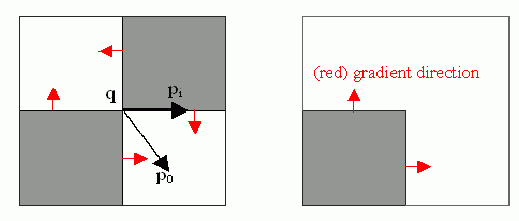
\includegraphics[width=1.0\textwidth]{pics/cornersubpix.png}

Sub-pixel accurate corner locator is based on the observation that every vector from the center $q$ to a point $p$ located within a neighborhood of $q$ is orthogonal to the image gradient at $p$ subject to image and measurement noise. Consider the expression:

\[
\epsilon_i = {DI_{p_i}}^T \cdot (q - p_i)
\]

where ${DI_{p_i}}$ is the image gradient at the one of the points $p_i$ in a neighborhood of $q$. The value of $q$ is to be found such that $\epsilon_i$ is minimized. A system of equations may be set up with $\epsilon_i$ set to zero:

\[
\sum_i(DI_{p_i} \cdot {DI_{p_i}}^T) - \sum_i(DI_{p_i} \cdot {DI_{p_i}}^T \cdot p_i)
\]

where the gradients are summed within a neighborhood ("search window") of $q$. Calling the first gradient term $G$ and the second gradient term $b$ gives:

\[
q = G^{-1} \cdot b
\]

The algorithm sets the center of the neighborhood window at this new center $q$ and then iterates until the center keeps within a set threshold.


\cvCppFunc{goodFeaturesToTrack}
Determines strong corners on an image.

\cvdefCpp{void goodFeaturesToTrack( const Mat\& image, vector<Point2f>\& corners,\par
                         int maxCorners, double qualityLevel, double minDistance,\par
                         const Mat\& mask=Mat(), int blockSize=3,\par
                         bool useHarrisDetector=false, double k=0.04 );}
\begin{description}
\cvarg{image}{The input 8-bit or floating-point 32-bit, single-channel image}
\cvarg{corners}{The output vector of detected corners}
\cvarg{maxCorners}{The maximum number of corners to return. If there are more corners than that will be found, the strongest of them will be returned}
\cvarg{qualityLevel}{Characterizes the minimal accepted quality of image corners; the value of the parameter is multiplied by the by the best corner quality measure (which is the min eigenvalue, see \cvCppCross{cornerMinEigenVal}, or the Harris function response, see \cvCppCross{cornerHarris}). The corners, which quality measure is less than the product, will be rejected. For example, if the best corner has the quality measure = 1500, and the \texttt{qualityLevel=0.01}, then all the corners which quality measure is less than 15 will be rejected.}
\cvarg{minDistance}{The minimum possible Euclidean distance between the returned corners}
\cvarg{mask}{The optional region of interest. If the image is not empty (then it needs to have the type \texttt{CV\_8UC1} and the same size as \texttt{image}), it will specify the region in which the corners are detected}
\cvarg{blockSize}{Size of the averaging block for computing derivative covariation matrix over each pixel neighborhood, see \cvCppCross{cornerEigenValsAndVecs}}
\cvarg{useHarrisDetector}{Indicates, whether to use \hyperref[cornerHarris]{Harris} operator or \cvCppCross{cornerMinEigenVal}}
\cvarg{k}{Free parameter of Harris detector}
\end{description}

The function finds the most prominent corners in the image or in the specified image region, as described
in \cite{Shi94}:
\begin{enumerate}
\item the function first calculates the corner quality measure at every source image pixel using the \cvCppCross{cornerMinEigenVal} or \cvCppCross{cornerHarris}
\item then it performs non-maxima suppression (the local maxima in $3\times 3$ neighborhood
are retained).
\item the next step rejects the corners with the minimal eigenvalue less than $\texttt{qualityLevel} \cdot \max_{x,y} qualityMeasureMap(x,y)$.
\item the remaining corners are then sorted by the quality measure in the descending order.
\item finally, the function throws away each corner $pt_j$ if there is a stronger corner $pt_i$ ($i < j$) such that the distance between them is less than \texttt{minDistance}
\end{enumerate}

The function can be used to initialize a point-based tracker of an object.

Note that the if the function is called with different values \texttt{A} and \texttt{B} of the parameter \texttt{qualityLevel}, and \texttt{A} > {B}, the vector of returned corners with \texttt{qualityLevel=A} will be the prefix of the output vector with \texttt{qualityLevel=B}.

See also: \cvCppCross{cornerMinEigenVal}, \cvCppCross{cornerHarris}, \cvCppCross{calcOpticalFlowPyrLK}, \cvCppCross{estimateRigidMotion}, \cvCppCross{PlanarObjectDetector}, \cvCppCross{OneWayDescriptor}

\cvCppFunc{HoughCircles}
Finds circles in a grayscale image using a Hough transform.

\cvdefCpp{void HoughCircles( Mat\& image, vector<Vec3f>\& circles,\par
                 int method, double dp, double minDist,\par
                 double param1=100, double param2=100,\par
                 int minRadius=0, int maxRadius=0 );}
\begin{description}
\cvarg{image}{The 8-bit, single-channel, grayscale input image}
\cvarg{circles}{The output vector of found circles. Each vector is encoded as 3-element floating-point vector $(x, y, radius)$}
\cvarg{method}{Currently, the only implemented method is \texttt{CV\_HOUGH\_GRADIENT}, which is basically \emph{21HT}, described in \cite{Yuen90}.}
\cvarg{dp}{The inverse ratio of the accumulator resolution to the image resolution. For example, if \texttt{dp=1}, the accumulator will have the same resolution as the input image, if \texttt{dp=2} - accumulator will have half as big width and height, etc}
\cvarg{minDist}{Minimum distance between the centers of the detected circles. If the parameter is too small, multiple neighbor circles may be falsely detected in addition to a true one. If it is too large, some circles may be missed}
\cvarg{param1}{The first method-specific parameter. in the case of \texttt{CV\_HOUGH\_GRADIENT} it is the higher threshold of the two passed to \cvCppCross{Canny} edge detector (the lower one will be twice smaller)}
\cvarg{param2}{The second method-specific parameter. in the case of \texttt{CV\_HOUGH\_GRADIENT} it is the accumulator threshold at the center detection stage. The smaller it is, the more false circles may be detected. Circles, corresponding to the larger accumulator values, will be returned first}
\cvarg{minRadius}{Minimum circle radius}
\cvarg{maxRadius}{Maximum circle radius}
\end{description}

The function finds circles in a grayscale image using some modification of Hough transform. Here is a short usage example:

\begin{lstlisting}
#include <cv.h>
#include <highgui.h>
#include <math.h>

using namespace cv;

int main(int argc, char** argv)
{
    Mat img, gray;
    if( argc != 2 && !(img=imread(argv[1], 1)).data)
        return -1;
    cvtColor(img, gray, CV_BGR2GRAY);
    // smooth it, otherwise a lot of false circles may be detected
    GaussianBlur( gray, gray, 9, 9, 2, 2 );
    vector<Vec3f> circles;
    houghCircles(gray, circles, CV_HOUGH_GRADIENT,
                 2, gray->rows/4, 200, 100 );
    for( size_t i = 0; i < circles.size(); i++ )
    {
         Point center(cvRound(circles[i][0]), cvRound(circles[i][1]));
         int radius = cvRound(circles[i][2]);
         // draw the circle center
         circle( img, center, 3, Scalar(0,255,0), -1, 8, 0 );
         // draw the circle outline
         circle( img, center, radius, Scalar(0,0,255), 3, 8, 0 );
    }
    namedWindow( "circles", 1 );
    imshow( "circles", img );
    return 0;
}
\end{lstlisting}

Note that usually the function detects the circles' centers well, however it may fail to find the correct radii. You can assist the function by specifying the radius range (\texttt{minRadius} and \texttt{maxRadius}) if you know it, or you may ignore the returned radius, use only the center and find the correct radius using some additional procedure.

See also: \cvCppCross{fitEllipse}, \cvCppCross{minEnclosingCircle}

\cvCppFunc{HoughLines}
Finds lines in a binary image using standard Hough transform.

\cvdefCpp{void HoughLines( Mat\& image, vector<Vec2f>\& lines,\par
                 double rho, double theta, int threshold,\par
                 double srn=0, double stn=0 );}
\begin{description}
\cvarg{image}{The 8-bit, single-channel, binary source image. The image may be modified by the function}
\cvarg{lines}{The output vector of lines. Each line is represented by a two-element vector $(\rho, \theta)$. $\rho$ is the distance from the coordinate origin $(0,0)$ (top-left corner of the image) and $\theta$ is the line rotation angle in radians ($0 \sim \textrm{vertical line}, \pi/2 \sim \textrm{horizontal line}$)}
\cvarg{rho}{Distance resolution of the accumulator in pixels}
\cvarg{theta}{Angle resolution of the accumulator in radians}
\cvarg{threshold}{The accumulator threshold parameter. Only those lines are returned that get enough votes ($>\texttt{threshold}$)}
\cvarg{srn}{For the multi-scale Hough transform it is the divisor for the distance resolution \texttt{rho}. The coarse accumulator distance resolution will be \texttt{rho} and the accurate accumulator resolution will be \texttt{rho/srn}. If both \texttt{srn=0} and \texttt{stn=0} then the classical Hough transform is used, otherwise both these parameters should be positive.}
\cvarg{stn}{For the multi-scale Hough transform it is the divisor for the distance resolution \texttt{theta}}
\end{description}

The function implements standard or standard multi-scale Hough transform algorithm for line detection. See \cvCppCross{HoughLinesP} for the code example.


\cvCppFunc{HoughLinesP}
Finds lines segments in a binary image using probabilistic Hough transform.

\cvdefCpp{void HoughLinesP( Mat\& image, vector<Vec4i>\& lines,\par
                  double rho, double theta, int threshold,\par
                  double minLineLength=0, double maxLineGap=0 );}
\begin{description}
\cvarg{image}{The 8-bit, single-channel, binary source image. The image may be modified by the function}
\cvarg{lines}{The output vector of lines. Each line is represented by a 4-element vector $(x_1, y_1, x_2, y_2)$, where $(x_1,y_1)$ and $(x_2, y_2)$ are the ending points of each line segment detected.}
\cvarg{rho}{Distance resolution of the accumulator in pixels}
\cvarg{theta}{Angle resolution of the accumulator in radians}
\cvarg{threshold}{The accumulator threshold parameter. Only those lines are returned that get enough votes ($>\texttt{threshold}$)}
\cvarg{minLineLength}{The minimum line length. Line segments shorter than that will be rejected}
\cvarg{maxLineGap}{The maximum allowed gap between points on the same line to link them.}
\end{description}

The function implements probabilistic Hough transform algorithm for line detection, described in \cite{Matas00}. Below is line detection example:

\begin{lstlisting}
/* This is a standalone program. Pass an image name as a first parameter
of the program.  Switch between standard and probabilistic Hough transform
by changing "#if 1" to "#if 0" and back */
#include <cv.h>
#include <highgui.h>
#include <math.h>

using namespace cv;

int main(int argc, char** argv)
{
    Mat src, dst, color_dst;
    if( argc != 2 || !(src=imread(argv[1], 0)).data)
        return -1;
        
    Canny( src, dst, 50, 200, 3 );
    cvtColor( dst, color_dst, CV_GRAY2BGR );    
        
#if 0
    vector<Vec2f> lines;
    HoughLines( dst, lines, 1, CV_PI/180, 100 );

    for( size_t i = 0; i < lines.size(); i++ )
    {
        float rho = lines[i][0];
        float theta = lines[i][1];
        double a = cos(theta), b = sin(theta);
        double x0 = a*rho, y0 = b*rho;
        Point pt1(cvRound(x0 + 1000*(-b)),
                  cvRound(y0 + 1000*(a)));
        Point pt2(cvRound(x0 - 1000*(-b)),
                  cvRound(y0 - 1000*(a)));
        line( color_dst, pt1, pt2, Scalar(0,0,255), 3, 8 );
    }
#else
    vector<Vec4i> lines;
    HoughLinesP( dst, lines, 1, CV_PI/180, 80, 30, 10 );
    for( size_t i = 0; i < lines.size(); i++ )
    {
        line( color_dst, Point(lines[i][0], lines[i][1]),
            Point(lines[i][2], lines[i][3]), Scalar(0,0,255), 3, 8 );
    }
#endif
    namedWindow( "Source", 1 );
    imshow( "Source", src );

    namedWindow( "Detected Lines", 1 );
    imshow( "Detected Lines", color_dst );

    waitKey(0);
    return 0;
}
\end{lstlisting}


This is the sample picture the function parameters have been tuned for:

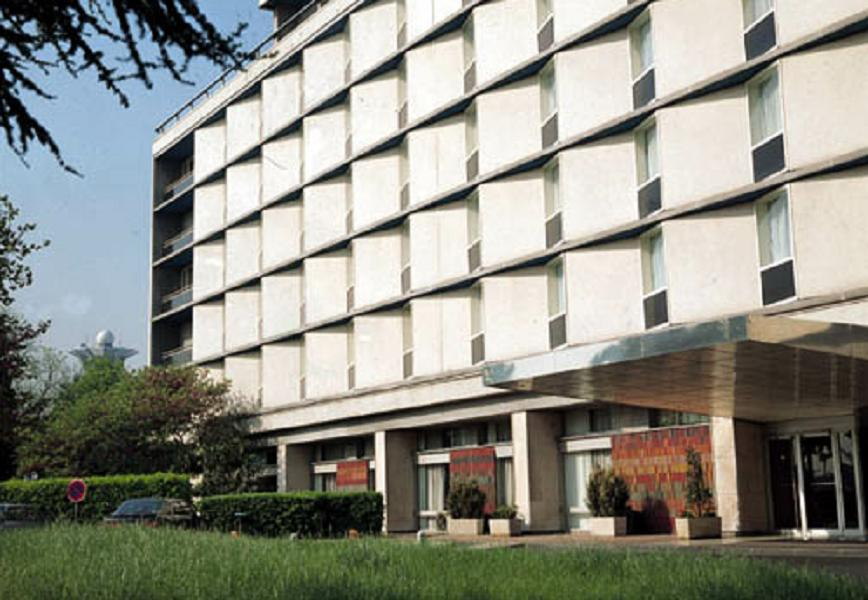
\includegraphics[width=0.5\textwidth]{pics/building.jpg}

And this is the output of the above program in the case of probabilistic Hough transform

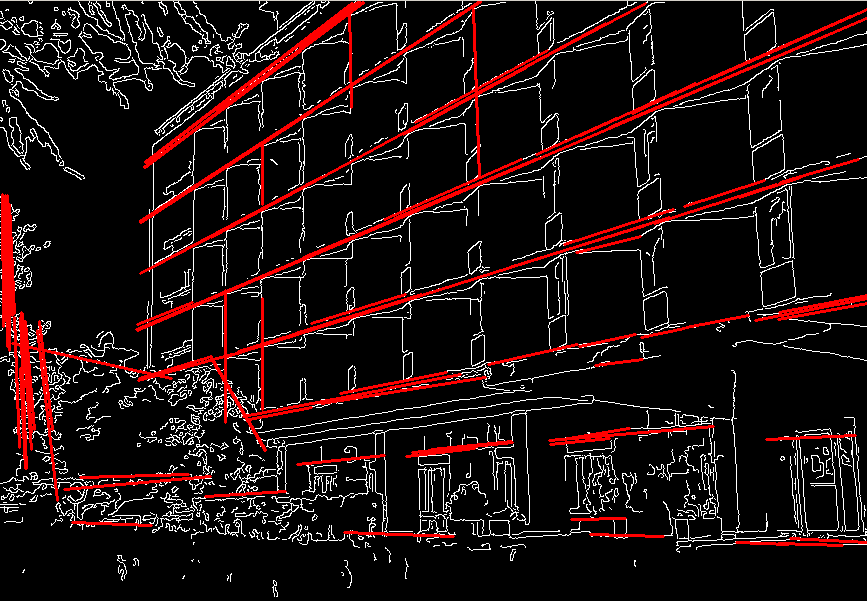
\includegraphics[width=0.5\textwidth]{pics/houghp.png}

\cvCppFunc{perCornerDetect}
Calculates the feature map for corner detection

\cvdefCpp{void preCornerDetect( const Mat\& src, Mat\& dst, int apertureSize,\par
                     int borderType=BORDER\_DEFAULT );}
\begin{description}
\cvarg{src}{The source single-channel 8-bit of floating-point image}
\cvarg{dst}{The output image; will have type \texttt{CV\_32F} and the same size as \texttt{src}}
\cvarg{apertureSize}{Aperture size of \cvCppCross{Sobel}}
\cvarg{borderType}{The pixel extrapolation method; see \cvCppCross{borderInterpolate}}
\end{description}

The function calculates the complex spatial derivative-based function of the source image

\[
\texttt{dst} = (D_x \texttt{src})^2 \cdot D_{yy} \texttt{src} + (D_y \texttt{src})^2 \cdot D_{xx} \texttt{src} - 2 D_x \texttt{src} \cdot D_y \texttt{src} \cdot D_{xy} \texttt{src}
\]

where $D_x$, $D_y$ are the first image derivatives, $D_{xx}$, $D_{yy}$ are the second image derivatives and $D_{xy}$ is the mixed derivative.

The corners can be found as local maximums of the functions, as shown below:

\begin{lstlisting}
Mat corners, dilated_corners;
preCornerDetect(image, corners, 3);
// dilation with 3x3 rectangular structuring element
dilate(corners, dilated_corners, Mat(), 1);
Mat corner_mask = corners == dilated_corners;
\end{lstlisting}


\cvCppFunc{KeyPoint}
Data structure for salient point detectors

\begin{lstlisting}
KeyPoint
{
public:
    // default constructor
    KeyPoint();
    // two complete constructors
    KeyPoint(Point2f _pt, float _size, float _angle=-1,
            float _response=0, int _octave=0, int _class_id=-1);
    KeyPoint(float x, float y, float _size, float _angle=-1,
             float _response=0, int _octave=0, int _class_id=-1);
    // coordinate of the point
    Point2f pt;
    // feature size
    float size;
    // feature orintation in degrees
    // (has negative value if the orientation
    // is not defined/not computed)
    float angle;
    // feature strength
    // (can be used to select only
    // the most prominent key points)
    float response;
    // scale-space octave in which the feature has been found;
    // may correlate with the size
    int octave;
    // point (can be used by feature
    // classifiers or object detectors)
    int class_id;
};

// reading/writing a vector of keypoints to a file storage
void write(FileStorage& fs, const string& name, const vector<KeyPoint>& keypoints);
void read(const FileNode& node, vector<KeyPoint>& keypoints);    
\end{lstlisting}


\cvCppFunc{MSER}
Maximally-Stable Extremal Region Extractor

\begin{lstlisting}
class MSER : public CvMSERParams
{
public:
    // default constructor
    MSER();
    // constructor that initializes all the algorithm parameters
    MSER( int _delta, int _min_area, int _max_area,
          float _max_variation, float _min_diversity,
          int _max_evolution, double _area_threshold,
          double _min_margin, int _edge_blur_size );
    // runs the extractor on the specified image; returns the MSERs,
    // each encoded as a contour (vector<Point>, see findContours)
    // the optional mask marks the area where MSERs are searched for
    void operator()(Mat& image, vector<vector<Point> >& msers, const Mat& mask) const;
};
\end{lstlisting}

The class encapsulates all the parameters of MSER (see \url{http://en.wikipedia.org/wiki/Maximally_stable_extremal_regions}) extraction algorithm. 

\cvCppFunc{SURF}
Class for extracting Speeded Up Robust Features from an image.

\begin{lstlisting}
class SURF : public CvSURFParams
{
public:
    // default constructor
    SURF();
    // constructor that initializes all the algorithm parameters
    SURF(double _hessianThreshold, int _nOctaves=4,
         int _nOctaveLayers=2, bool _extended=false);
    // returns the number of elements in each descriptor (64 or 128)
    int descriptorSize() const;
    // detects keypoints using fast multi-scale Hessian detector
    void operator()(const Mat& img, const Mat& mask,
                    vector<KeyPoint>& keypoints) const;
    // detects keypoints and computes the SURF descriptors for them
    void operator()(const Mat& img, const Mat& mask,
                    vector<KeyPoint>& keypoints,
                    vector<float>& descriptors,
                    bool useProvidedKeypoints=false) const;
};
\end{lstlisting}

The class \texttt{SURF} implements Speeded Up Robust Features descriptor \cite{Bay06}.
There is fast multi-scale Hessian keypoint detector that can be used to find the keypoints
(which is the default option), but the descriptors can be also computed for the user-specified keypoints.
The function can be used for object tracking and localization, image stitching etc. See the
\texttt{find\_obj.cpp} demo in OpenCV samples directory.


\cvCppFunc{StarDetector}
Implements Star keypoint detector

\begin{lstlisting}
class StarDetector : CvStarDetectorParams
{
public:
    // default constructor
    StarDetector();
    // the full constructor initialized all the algorithm parameters:
    // maxSize - maximum size of the features. The following 
    //      values of the parameter are supported:
    //      4, 6, 8, 11, 12, 16, 22, 23, 32, 45, 46, 64, 90, 128
    // responseThreshold - threshold for the approximated laplacian,
    //      used to eliminate weak features. The larger it is,
    //      the less features will be retrieved
    // lineThresholdProjected - another threshold for the laplacian to 
    //      eliminate edges
    // lineThresholdBinarized - another threshold for the feature 
    //      size to eliminate edges.
    // The larger the 2 threshold, the more points you get.
    StarDetector(int maxSize, int responseThreshold,
                 int lineThresholdProjected,
                 int lineThresholdBinarized,
                 int suppressNonmaxSize);

    // finds keypoints in an image
    void operator()(const Mat& image, vector<KeyPoint>& keypoints) const;
};
\end{lstlisting}

The class implements a modified version of CenSurE keypoint detector described in
\cite{Agrawal08}

\fi
